\documentclass[11pt,letterpaper]{article}

% Preamble for Position Paper
% Standard packages for formatting and layout
\usepackage[margin=1in]{geometry}
\usepackage{graphicx}
\usepackage[colorlinks=true,linkcolor=blue,citecolor=blue,urlcolor=blue]{hyperref}
\usepackage{booktabs}
\usepackage[dvipsnames]{xcolor}
\usepackage{amsmath,amssymb}
\usepackage{caption}
\usepackage{subcaption}
\usepackage{cleveref}

% Bibliography
\usepackage[numbers,sort&compress]{natbib}
\bibliographystyle{unsrtnat}

% Line spacing
\usepackage{setspace}
\onehalfspacing

% Section formatting
\usepackage{titlesec}
\titleformat{\section}{\Large\bfseries}{\thesection}{1em}{}
\titleformat{\subsection}{\large\bfseries}{\thesubsection}{1em}{}

% Custom commands
\newcommand{\gap}[1]{\textbf{\textcolor{RedOrange}{Gap #1}}}
\newcommand{\keyword}[1]{\textit{#1}}
\newcommand{\psup}{\textcolor{YellowOrange}{$\boldsymbol{\circ}$}}  % partial support
\newcommand{\nsup}{\texttimes}  % no support
\newcommand{\fsup}{\checkmark}  % full support

% Figure path
\graphicspath{{./figures/}}

% Better list spacing
\usepackage{enumitem}
\setlist{nosep}


\title{\textbf{Beyond SMILES: Evaluating Agentic AI for Drug Discovery}}

\author{Edward Wijaya\\
\small StemRIM, Inc. \\
\small \texttt{wijaya@stemrim.com}}

\date{}

\begin{document}

\maketitle

\begin{abstract}
Agentic AI systems like ChatInvent and Coscientist demonstrate impressive capabilities but reveal systematic blind spots when applied beyond small-molecule workflows at well-resourced pharmaceutical companies. Drawing on experience leading 14+ AI-driven drug discovery projects at a small biotech specializing in therapeutic peptides, this perspective identifies five critical gaps: the small molecule bias excluding protein language models and peptide-specific property prediction; the absence of in vivo to in silico bridges for longitudinal, multi-modal animal data; LLM-centric orchestration that excludes machine learning training, reinforcement learning, and multi-paradigm coordination; resource-abundant design assumptions mismatched to small biotech realities of limited data and modest compute; and single-metric optimization ignoring multi-objective trade-offs in safety, efficacy, and stability. Each gap is illustrated through practitioner experience spanning peptide generation, behavioral phenotyping, multi-endpoint prediction, and longitudinal in vivo modeling. We propose five design principles: multi-paradigm orchestration treating ML training and RL as architectural primitives, modality-aware architectures supporting peptides and biologics, in vivo integration through temporal modeling and causal inference, data-efficient learning via transfer and active learning, and multi-objective optimization with uncertainty quantification and Pareto visualization. The goal is building computational partners that augment practitioner judgment, not replacing human expertise, and that can operate under realistic data, modality, and resource constraints.

\end{abstract}

\section{Introduction: The Promise vs Reality of Agentic AI in Drug Discovery}
\label{sec:introduction}

\subsection{The Current Narrative}

The past three years have witnessed an explosion of agentic AI systems targeting drug discovery workflows. In late 2023, Coscientist demonstrated autonomous chemical synthesis planning and execution \citep{boiko2023coscientist}, while ChemCrow showed how GPT-4 could orchestrate 18 chemistry tools for synthesis route optimization and safety assessment \citep{bran2023chemcrow}. More recently, ChatInvent completed a 13-month deployment at AstraZeneca, performing literature synthesis and hypothesis generation at scale \citep{he2026chatinvent}. PharmAgents extended this paradigm to integrate knowledge graphs with large language model reasoning for target identification and compound prioritization \citep{swanson2024pharmagents}, while systems like MADD and DiscoVerse promise multi-agent collaboration for end-to-end drug design.

These demonstrations have catalyzed excitement across the pharmaceutical industry. The dominant narrative positions agentic AI as the next frontier in computational drug discovery, moving beyond static prediction models to systems that can autonomously navigate literature, design experiments, and propose hypotheses. Industry editorials proclaim an "agentic era" where AI systems will act as collaborators rather than tools \citep{lakhan2025agentic}. Comprehensive technical surveys map an expanding landscape of agent architectures, tool integrations, and capability benchmarks \citep{seal2025aiagents}.

The architectural pattern underlying most current systems is remarkably consistent: a large language model serves as the central orchestrator, decomposing complex queries into tool calls, synthesizing results, and generating natural language explanations. ChemCrow's GPT-4 backbone routes requests to RDKit for molecular property calculation, PubChem for database searches, and specialized APIs for reaction prediction. ChatInvent mines scientific literature to identify research gaps and suggest experimental directions. Coscientist interfaces with laboratory automation platforms to translate synthesis plans into executable protocols.

This LLM-centric design has proven effective for tasks that map naturally to text-based reasoning: literature review, synthesis route enumeration, protocol documentation, and safety datasheet analysis. The systems excel when the knowledge required exists in their training corpora or can be retrieved through search, and when the outputs are text or simple API calls to well-defined computational tools.

\subsection{The Gap: What Happens Outside the Lab Automation Paradigm}

However, a closer examination of these systems reveals systematic blind spots. Current agentic AI architectures are optimized for a specific context: small-molecule drug discovery, target-based screening workflows, high-throughput in vitro assays, and well-resourced pharmaceutical companies with extensive computational infrastructure and large datasets. When applied outside this design envelope, to peptide therapeutics, in vivo efficacy modeling, or resource-constrained small biotechs, the limitations become stark.

Consider the problem of therapeutic peptide design for regenerative medicine. Unlike small molecules represented as SMILES strings with well-defined chemical properties, peptides are sequences of 5 to 50 amino acids with complex conformational dynamics, aggregation propensities, protease vulnerabilities, and immunogenic epitopes. The structure-activity relationships that govern peptide bioactivity do not transfer from small-molecule experience. Stability optimization requires modeling peptide-enzyme interactions across dozens of protease families. Receptor binding prediction demands protein language models like ESM-2 \citep{lin2023esm2} or ProtBERT \citep{elnaggar2021protbert}, not molecular fingerprints. Yet no current agent architecture provides native support for protein language model fine-tuning, conformational sampling, or aggregation prediction.

The disconnect becomes more pronounced when moving from in vitro screens to in vivo efficacy studies. Animal models generate longitudinal data across multiple modalities: behavioral scores tracked over weeks, tissue histology captured through imaging, transcriptomic responses measured via RNA sequencing, and clinical observations recorded in semi-structured notes. In a traumatic brain injury model, efficacy might manifest as improved motor coordination at day 7, reduced neuroinflammation at day 14, and enhanced neurogenesis at day 28, all correlated with behavioral phenotypes quantified through computer vision analysis of animal movement patterns. No existing agent system can integrate these heterogeneous, temporal data streams to predict long-term therapeutic outcomes or identify mechanistic signatures.

The assumption of abundant computational resources and large datasets further limits applicability. ChatInvent's deployment at AstraZeneca presumes access to institutional literature subscriptions, high-performance computing clusters, and proprietary compound libraries numbering in the millions. A small biotech developing peptide therapeutics might have 50 to 500 proprietary sequences tested across a handful of assays, a single GPU workstation, and a team where the same person designs experiments, runs machine learning models, and analyzes results. Transfer learning, few-shot adaptation, and batch-mode automation become essential rather than optional, yet current agent architectures provide no systematic support for these capabilities.

Perhaps most fundamentally, real drug discovery requires navigating multi-objective trade-offs under uncertainty. A candidate peptide might show tenfold higher bioactivity than alternatives but with a narrower safety margin, increased aggregation propensity, or reduced proteolytic stability. The optimal choice depends on the development stage, risk tolerance, and specific therapeutic context. Current agents optimize single metrics or treat multi-objective problems as weighted sums, ignoring the Pareto frontier structure of real design spaces and providing no support for uncertainty quantification or sensitivity analysis.

The gap between capability demonstrations and practitioner reality creates a fundamental question: how must agent architectures evolve to address therapeutic modalities beyond small molecules, data contexts beyond high-throughput screening, computational paradigms beyond LLM tool-calling, resource constraints beyond large pharma budgets, and decision frameworks beyond single-objective optimization? This paper draws on experience leading 14+ AI-driven projects spanning machine learning for multi-endpoint bioactivity prediction, generative peptide design with protein language models, reinforcement learning for sequence optimization, longitudinal in vivo efficacy modeling, behavioral phenotyping through computer vision, RNA sequencing analysis, and multi-objective safety versus efficacy navigation. Each project revealed architectural assumptions in current agent systems that do not generalize. Understanding these gaps is essential for building the next generation of computational partners in drug discovery.

The following sections identify five critical blind spots: the small molecule bias in tool design and model integration (\S\ref{sec:small-molecule}), the absence of in vivo to in silico bridges (\S\ref{sec:invivo}), the limitations of LLM-centric multi-agent orchestration (\S\ref{sec:multiparadigm}), the mismatch with small biotech realities (\S\ref{sec:smallbiotech}), and the single-metric optimization trap (\S\ref{sec:multiobjective}). We conclude with a practitioner's wishlist (\S\ref{sec:wishlist}) proposing concrete design principles for agent systems that can serve as true computational partners rather than sophisticated chatbots.


\section{Evaluation Framework}
\label{sec:methods}

This section describes the systematic approach used to evaluate agentic AI frameworks against drug discovery task requirements.

\subsection{Agent Framework Selection}

We selected six agentic AI frameworks representing distinct design paradigms in drug discovery automation (Table~\ref{tab:frameworks}). Selection criteria required published or preprint documentation with sufficient architectural detail, demonstrated application to drug discovery tasks, and representation of distinct paradigms (single-agent, multi-agent, tool-augmented).

\begin{table}[htbp]
\centering
\caption{Agentic AI Frameworks Evaluated}
\label{tab:frameworks}
\small
\begin{tabular}{llll}
\hline
\textbf{Framework} & \textbf{Year} & \textbf{Organization} & \textbf{Primary Focus} \\
\hline
ChemCrow \citep{bran2024chemcrow} & 2023 & EPFL/Rochester & Chemistry tool orchestration \\
Coscientist \citep{boiko2023coscientist} & 2023 & CMU & Autonomous synthesis \\
PharmAgents \citep{gao2025pharmagents} & 2025 & Tsinghua & Target-compound interaction \\
ChatInvent \citep{he2026chatinvent} & 2026 & AstraZeneca & Literature-driven hypothesis \\
MADD \citep{madd2025} & 2025 & Multi-institutional & Multi-agent drug design \\
DiscoVerse \citep{discoverse2025} & 2025 & Roche & Discovery workflow automation \\
\hline
\end{tabular}
\end{table}

\subsection{Task Class Definition}

We defined 15 task classes derived from real-world drug discovery workflows spanning peptide therapeutics, in vivo pharmacology, and computational biology. These task classes represent the computational requirements encountered across 14 projects at a small biotech specializing in therapeutic peptides for regenerative medicine:

\begin{enumerate}
\item ML bioactivity prediction (multi-endpoint regression)
\item Generative peptide design (PLM fine-tuning)
\item Peptide-receptor binding site analysis and clustering
\item In vivo recovery modeling (longitudinal clinical scores)
\item Peptide-enzyme interaction modeling for stability optimization
\item Protein language model-based receptor type prediction
\item Monte Carlo optimization for peptide landscape exploration
\item RNA sequencing and single-cell transcriptomics analysis
\item Digital image processing for tissue quantification
\item Immune response profiling (pathway analysis)
\item Functional annotation and pathway enrichment
\item Computer vision for behavioral phenotyping
\item Predictive modeling bridging in vivo and in vitro endpoints
\item Reinforcement learning for de novo peptide generation
\item Safety and toxicology modeling (dose-response, multi-objective trade-offs)
\end{enumerate}

These task classes span the full discovery pipeline from target identification through preclinical validation, representing computational requirements that extend well beyond the small-molecule, target-based workflows that current frameworks primarily support.

\subsection{Evaluation Dimensions}

Each framework was evaluated across five dimensions capturing distinct aspects of drug discovery computational requirements:

\begin{enumerate}
\item \textbf{Molecular representation coverage:} Support for peptides, proteins, and biologics beyond SMILES strings and molecular fingerprints.
\item \textbf{Computational paradigm support:} Capacity for ML training, reinforcement learning, simulation, and constrained optimization beyond LLM inference and API calls.
\item \textbf{Data modality integration:} Handling of in vivo longitudinal data, imaging, transcriptomics, and behavioral data beyond text and tabular formats.
\item \textbf{Resource assumptions:} Alignment with varying data volumes, compute budgets, and team sizes, particularly resource-constrained settings.
\item \textbf{Optimization framework:} Support for multi-objective optimization, uncertainty quantification, and constraint satisfaction beyond single-metric objectives.
\end{enumerate}

\subsection{Analysis Approach}

For each framework-task pair, we performed a binary capability assessment (supported or not supported) based on published documentation, source code availability, and demonstrated use cases. We computed a coverage score as the fraction of 15 task classes addressable per framework. Gaps were identified as task classes with zero or minimal framework coverage. Design requirements were derived from the capabilities needed to close identified gaps, grounded in practitioner experience with the corresponding task classes.

This approach has limitations: binary assessment may oversimplify nuanced partial support, and the rapidly evolving nature of the field means new frameworks may address some identified gaps. We discuss these limitations further in \S\ref{sec:discussion}.


\section{Results: Five Capability Gaps}
\label{sec:results}

Table~\ref{tab:capability-matrix} presents the core result of our evaluation: a capability matrix mapping 15 task classes against six agentic AI frameworks. Coverage is sparse. No framework fully supports any of the 15 task classes. Partial support, where a framework provides adjacent functionality that does not address the task-specific requirements, appears in only a few cases. The five gaps identified in the following subsections emerge directly from this matrix: clusters of zero-coverage task classes that share underlying architectural limitations.

\begin{table}[htbp]
\centering
\caption{Capability Matrix: Six Frameworks Evaluated Against 15 Task Classes. \fsup\ = supported, \psup\ = partial (adjacent capability exists but does not meet task requirements), \nsup\ = not supported. Coverage scores count \fsup\ as 1 and \psup\ as 0.5. CC = ChemCrow, CS = Coscientist, PA = PharmAgents, CI = ChatInvent, MA = MADD, DV = DiscoVerse.}
\label{tab:capability-matrix}
\small
\begin{tabular}{clccccccc}
\toprule
\textbf{\#} & \textbf{Task Class} & \textbf{CC} & \textbf{CS} & \textbf{PA} & \textbf{CI} & \textbf{MA} & \textbf{DV} & \textbf{Gap} \\
\midrule
1 & ML bioactivity prediction & \nsup & \nsup & \psup & \nsup & \psup & \psup & 3 \\
2 & Generative peptide design & \nsup & \nsup & \nsup & \nsup & \nsup & \nsup & 1 \\
3 & Peptide-receptor binding & \psup & \nsup & \psup & \nsup & \psup & \nsup & 1 \\
4 & In vivo recovery modeling & \nsup & \nsup & \nsup & \nsup & \nsup & \nsup & 2 \\
5 & Peptide-enzyme stability & \nsup & \nsup & \nsup & \nsup & \nsup & \nsup & 1 \\
6 & PLM receptor prediction & \nsup & \nsup & \nsup & \nsup & \nsup & \nsup & 1 \\
7 & Monte Carlo optimization & \nsup & \nsup & \nsup & \nsup & \nsup & \nsup & 1,3 \\
8 & RNA-seq / scRNA-seq & \nsup & \nsup & \nsup & \nsup & \nsup & \nsup & 2 \\
9 & Image-based quantification & \nsup & \nsup & \nsup & \nsup & \nsup & \nsup & 2 \\
10 & Immune response profiling & \nsup & \nsup & \psup & \psup & \nsup & \psup & 2 \\
11 & Functional annotation & \nsup & \nsup & \psup & \psup & \nsup & \psup & 2 \\
12 & Behavioral phenotyping & \nsup & \nsup & \nsup & \nsup & \nsup & \nsup & 2 \\
13 & In vivo/in vitro bridging & \nsup & \nsup & \nsup & \nsup & \nsup & \nsup & 2 \\
14 & RL peptide generation & \nsup & \nsup & \nsup & \nsup & \nsup & \nsup & 1,3 \\
15 & Safety/toxicology (multi-obj) & \psup & \nsup & \psup & \psup & \psup & \psup & 5 \\
\midrule
\multicolumn{2}{l}{\textbf{Coverage (\%)}} & \textbf{6.7} & \textbf{0.0} & \textbf{16.7} & \textbf{10.0} & \textbf{10.0} & \textbf{13.3} & \\
\bottomrule
\end{tabular}
\vspace{4pt}

\footnotesize
\textbf{Partial support notes:} Task 1: frameworks invoke pre-trained predictors but cannot train, validate, or tune models on proprietary data. Task 3: small-molecule docking tools exist but do not handle peptide conformational flexibility. Tasks 10--11: knowledge graph queries or literature synthesis provide pathway-level information but not computational enrichment pipelines (GSEA, upstream regulator analysis). Task 15: toxicophore flagging or ADMET prediction for small molecules; no multi-objective trade-off reasoning or dose-response modeling.
\end{table}


\subsection{Gap 1: Small-Molecule Representation Bias}
\label{sec:small-molecule}

Current agentic systems are architected around small molecules: SMILES strings, docking scores, synthetic accessibility metrics, and retrosynthesis planning. This works for medicinal chemistry but breaks down for peptide therapeutics requiring fundamentally different computational approaches.

\subsubsection{Findings}

All six frameworks evaluated assume small-molecule representations (SMILES strings, molecular fingerprints, docking scores). Task classes 2, 3, 5, 6, and 7 (peptide-specific workflows) receive zero coverage across all frameworks. No framework supports protein language models (ProtBERT, ESM-2, ProGen) as first-class components for sequence-based therapeutics design.

\subsubsection{The Peptide-Specific Challenge Space}

Therapeutic peptides (2 to 50 amino acids) bridge small molecules and biologics. Unlike rigid small molecules, peptides are conformationally flexible, sampling diverse structural states. They achieve high selectivity through induced-fit binding but face aggregation, protease degradation, and permeability barriers. These challenges extend beyond peptides to biologics broadly: antibodies require CDR loop modeling, nanobodies need single-domain folding, and fusion proteins demand multi-domain interaction prediction. The small-molecule bias is a biologics-wide limitation.

Peptide discovery diverges from small-molecule workflows. Structure-activity relationships do not transfer; conservative substitutions can abolish activity while drastic changes improve potency. Stability dominates. Developing peptides for traumatic brain injury, efficacy-stability trade-offs exceeded potency concerns. A bioactive peptide with minute-scale serum half-life has no therapeutic value. Protease resistance requires modeling interactions across dozens of enzyme families. Immunogenicity demands epitope scanning and MHC binding prediction. Aggregation depends on charge distribution and hydrophobic patterning.

Current agents provide no pathway for these requirements. ChemCrow includes RDKit, which does not handle peptide conformational sampling. PharmAgents focuses on small-molecule structure-based design workflows not designed for flexible peptide interactions. ChatInvent mines small-molecule synthesis routes and molecular design, irrelevant to peptide synthesis.

Practitioners encounter immediate friction. SMILES encoding of peptides is error-prone, risking loss of stereochemical and conformational information, particularly for non-natural amino acids. Standard molecular fingerprints (Morgan, MACCS) perform poorly on peptides, which lack equivalent standard representations. Rigid-molecule docking produces unreliable scores. Retrosynthesis metrics are meaningless. Even data storage becomes awkward: sequence variants, post-translational modifications, and assay metadata rarely fit small-molecule databases designed for single canonical structures.

\subsubsection{Protein Language Models vs Molecular Fingerprints}

\begin{figure}[htbp]
\centering
\includegraphics[width=\textwidth]{figures/fig2-workflow-complexity.jpeg}
\caption{Workflow Complexity: Small Molecules vs Peptides. Top: Small molecule workflow follows a linear path from SMILES representation through RDKit property calculation to docking. Bottom: Peptide workflow branches into multiple parallel analysis streams including structural prediction, aggregation propensity, stability, immunogenicity, membrane permeability, and protease resistance, requiring integration of diverse computational tools and protein language models.}
\label{fig:workflow-complexity}
\end{figure}

Protein language models define peptide design. ProtBERT \citep{elnaggar2022protbert}, ESM-2 \citep{lin2023esm2}, and ProGen \citep{madani2023progen} encode evolutionary and structural priors from millions of protein sequences. ESM-2 embeddings predict receptor types from sequence alone. ProtBERT fine-tuning enables transfer learning from limited labeled data, often requiring only hundreds of examples for task-specific classifiers.

Peptide-aware models are emerging. PepTune \citep{peptune2024} uses a masked discrete diffusion model with Monte Carlo Tree Guidance for multi-objective peptide generation, optimizing across binding affinity, permeability, and stability simultaneously. PepMLM \citep{pepmlm2025} fine-tunes ESM-2 to design peptide binders conditioned on target protein sequences, with experimental validation on disease-relevant targets. These are real advances in peptide-specific modeling. However, they are standalone tools, not components of agentic workflows. No current system chains peptide generation with proprietary fine-tuning, active learning, iterative design-test cycles, or multi-endpoint optimization in closed loops. The gap is workflow integration, not individual capability.

Building peptide workflows requires capabilities current agents lack. Developing a receptor binding classifier involves curating training sets, extracting ESM-2 embeddings, training supervised classifiers, validating performance, and iterating hyperparameters. This is gradient-based ML, not API calls. The work also depends on small, noisy datasets where careful cross-validation and calibration matter more than single headline metrics. Agents must expose these uncertainties clearly so biologists can prioritize synthesis and testing. Without that, the workflow reverts to manual triage and ad hoc heuristics.
No current system supports this autonomously. LLM orchestrators assume models are black-box inference APIs. There is no fine-tuning support, dataset version control, or hyperparameter search. Agents retrieve embeddings but cannot adjust attention heads or train task-specific classifiers on proprietary data.

Generative modeling extends this gap. ProtGPT2 \citep{ferruz2022protgpt2} fine-tunes on therapeutic sequences for de novo generation. Reinforcement learning optimizes multi-objective reward functions combining bioactivity and stability, requiring reward models, policy networks, gradients, and KL regularization. These ML workflows requiring end-to-end training control exceed current agent architectures.

The gap reflects a missing paradigm, not a missing tool. Protein language models are the foundation of peptide discovery, demanding first-class support for training and fine-tuning. Without this, agents cannot support the core workflows practitioners use to move from sequence space exploration to experimentally validated leads.

\subsubsection{Derived Requirements}

Peptide-aware architectures require protein language models as core components, not external APIs. First, fine-tuning pipelines: dataset curation, train-validation-test splits, learning rate scheduling, early stopping, checkpointing. Agents should fine-tune ProtBERT on 200 sequences and return calibrated classifiers with uncertainty estimates.

Second, structural biology integration. AlphaFold \citep{jumper2021alphafold} structure prediction is central to peptide design. Flexible docking requires conformational sampling. Molecular dynamics provides stability and kinetics insights. These tools must integrate into multi-step workflows and feed back into sequence optimization, not sit as isolated analyses.

Third, multi-objective optimization. Peptide design balances bioactivity, stability, selectivity, and immunogenicity. We used curriculum learning for in vivo efficacy: initially rewarding bioactivity improvements, then progressively adding stability and toxicity constraints. This prevented local optima and maintained diversity. Current agents provide no framework for multi-stage optimization.

Fourth, diversity-aware generation. Generative models suffer mode collapse, producing reward-maximizing sequences with little variety. Practitioners use diversity penalties and max-min rewards, requiring state maintenance and dynamic sampling. LLM agents treat tool calls as stateless.

Finally, active learning loops. Limited budgets require careful peptide selection. Active learning maximizes information gain by prioritizing uncertain predictions. This requires uncertainty quantification, acquisition functions, and feedback loops updating models across multiple rounds.

Peptide discovery is a distinct paradigm requiring ML training, structural biology, and multi-objective optimization as core capabilities. It also requires sequence-aware data management: tracking modifications, synthesis constraints, and assay provenance across iterative cycles. The small-molecule bias reflects architectural assumptions that must be revisited.


\subsection{Gap 2: Absence of In Vivo-In Silico Integration}
\label{sec:invivo}

The absence of in vivo modeling is a fundamental gap. Current agents excel at in vitro automation: Coscientist plans syntheses \citep{boiko2023coscientist}, ChemCrow screens compound libraries, ChatInvent mines literature. But critical validation happens in vivo, where candidates confront pharmacokinetics, biodistribution, metabolism, toxicology, and long-term efficacy unpredictable from binding affinity.

Animal studies generate a distinct class of data: longitudinal (days to months), multi-modal (behavioral scores, imaging, molecular profiling), noisy (biological variability dwarfs plate assay precision), low-throughput (tens of compounds, not thousands), and expensive. These characteristics make in vivo the bottleneck, yet agents provide no pathway to incorporate this data.

\subsubsection{Findings}

Task classes 4, 9, 12, and 13 (in vivo and imaging tasks) receive zero coverage across all six frameworks. All frameworks terminate at in vitro automation or literature-based hypothesis generation. No framework supports longitudinal data modeling, multi-modal fusion, or causal inference from animal study data.

\subsubsection{The Lab Automation Ceiling}

Lab automation reaches a hard ceiling at in vivo studies. Synthesis platforms and high-throughput screening test thousands of compounds daily. But animal experiments cannot be scaled or automated, requiring specialized facilities, personnel, ethical oversight, and weeks of time.

An agent might design a peptide and predict binding, but cannot integrate a 28-day traumatic brain injury study measuring behavioral recovery, histological regeneration, and transcriptomic neuroprotection. Data formats, temporal structure, and statistical requirements exceed current capabilities.

In vivo studies yield heterogeneous streams. Neurological injury evaluation includes behavioral assessments (motor coordination via beam walking, generating ordinal scores), tissue histology (cell proliferation requiring computer vision), RNA sequencing (high-dimensional gene expression needing differential expression and pathway enrichment), and clinical notes (semi-structured weight and adverse events). This multi-modal integration remains outside current agent scope.

Developing composite efficacy metrics exposed this gap. A peptide increasing cell proliferation threefold in vitro shows temporal in vivo dynamics: inflammatory response (days 1-3), progenitor proliferation (days 7-10), functional recovery (day 28). Predicting sustained benefit requires temporal modeling, dataset curation, feature engineering, and validation outside LLM tool-calling scope.

\subsubsection{Multi-Modal, Longitudinal Data Integration}

\begin{figure}[htbp]
\centering
\includegraphics[width=\textwidth]{figures/fig3-invivo-insilico-gap.jpeg}
\caption{What Agents Can and Cannot Process. Matrix showing data types on the vertical axis and agent accessibility on the horizontal axis. Green checkmarks indicate data types current agents handle well (text, SMILES, PDB files, CSV data, literature). Red X marks denote data types agents struggle with (behavioral videos, clinical score trajectories, tissue imaging, multi-modal transcriptomics, longitudinal measurements with dropout). This visualization reveals the systematic exclusion of in vivo data modalities from current agent architectures.}
\label{fig:invivo-gap}
\end{figure}

The core challenge is that in vivo data does not fit the tidy CSV format that machine learning pipelines expect (Table~\ref{tab:data-accessibility}). Behavioral scores are ordinal and subject to inter-rater variability.

\begin{table}[htbp]
\centering
\caption{Data Type Accessibility for Current Agent Systems}
\label{tab:data-accessibility}
\begin{tabular}{lllp{4cm}}
\hline
\textbf{Data Type} & \textbf{Format} & \textbf{Agent-Readable} & \textbf{Example Use Case} \\
\hline
SMILES strings & Text & Yes & Small molecule property prediction \\
Literature abstracts & Text & Yes & Knowledge synthesis \\
PDB structures & Structured & Yes & Protein structure analysis \\
CSV assay data & Tabular & Yes & High-throughput screening \\
Behavioral videos & Video & No & Phenotyping analysis \\
Clinical trajectories & Time-series & Partial & Longitudinal efficacy modeling \\
Tissue imaging & Image & Partial & Histological quantification \\
RNA-seq data & FASTQ/BAM & No & Transcriptomic profiling \\
Clinical notes & Semi-structured text & Partial & Adverse event detection \\
\hline
\end{tabular}
\end{table}

Behavioral phenotyping via DeepLabCut \citep{mathis2018deeplabcut} tracks animal poses in videos, generating time-series keypoint coordinates. Computing behavioral metrics (inter-animal distance, contact time, grooming) requires training pose estimation, validating tracking, computing features, and statistical testing. Practitioners must handle this workflow manually, spanning video processing, supervised learning, time-series engineering, and hypothesis testing.

RNA-seq requires quality control, alignment, and quantification into expression matrices. Differential expression identifies treatment effects. Pathway enrichment maps genes to biological processes via KEGG \citep{kanehisa2023kegg} or Gene Ontology. Upstream regulator analysis infers transcription factors driving changes. The FASTQ-to-hypothesis pipeline needs bioinformatics tools (STAR, HISAT2, DESeq2, edgeR, GSEA \citep{subramanian2005gsea}) that agents do not integrate. Recent systems like Medea \citep{medea2026} have begun addressing multi-omics analysis agenically, handling transcriptomics, protein networks, and pathway analysis. However, these process static datasets rather than longitudinal in vivo time-series, and do not integrate behavioral phenotyping, imaging, or temporal efficacy modeling.

Integrating heterogeneous sources for predictive biomarkers is valuable yet absent. Correlating in vitro bioactivity with in vivo efficacy required extracting features from multiple assays, normalizing across scales, aligning with temporal data (days 3, 7, 14, 28), and training regression models predicting long-term outcomes. This workflow involved feature engineering, imputation, stratified cross-validation, and model selection; these are ML workflows, not LLM reasoning.

\subsubsection{Safety, Efficacy, and Translation}

In vivo models surface safety-efficacy trade-offs that in silico screens miss. Tenfold bioactivity increases may trigger immune activation or hepatotoxicity. Stability modifications (D-amino acids, cyclization) may reduce affinity or increase aggregation.

Toxicology requires dose-response analysis via generalized linear mixed models accounting for repeated measures and time-dependent effects. Identifying therapeutic windows where efficacy plateaus but toxicity remains acceptable is essential. Species translation compounds this: mouse pharmacokinetics extrapolate to humans via allometric scaling, but peptide stability varies by species protease expression and rodent-tolerated peptides may provoke primate antibody responses. Agents cannot construct dose-response curves, compute LD50 confidence intervals, or model cross-species translation uncertainties. We return to the broader multi-objective trade-offs these challenges imply in \S\ref{sec:multiobjective}.

\subsubsection{Derived Requirements}

Closing the in vivo-in silico gap requires three capabilities absent from current frameworks. First, temporal state-space models for longitudinal in vivo trajectories that capture treatment dynamics across days to weeks. Second, causal inference tools (do-calculus, counterfactual reasoning) to separate correlation from mechanism in complex biological systems. Third, multi-modal data fusion integrating clinical scores, imaging, transcriptomics, and behavioral data into unified predictive models. Until agents ingest longitudinal scores, integrate transcriptomics, quantify dose-response uncertainty, and navigate multi-objective trade-offs under biological variability, utility remains confined to early hit identification. Most development cost and risk lies in translating in vitro activity to in vivo efficacy and safety \citep{dimasi2016costs}.


\input{sections/05-gap-multi-paradigm.tex}

\subsection{Gap 4: Misalignment with Small-Biotech Constraints}
\label{sec:smallbiotech}

ChatInvent's deployment at AstraZeneca \citep{he2026chatinvent} accessed institutional databases, HPC clusters, and proprietary libraries built over decades, with specialized teams (medicinal chemists, computational chemists, biologists, data scientists). This large pharma context defines current agent design assumptions but is not representative.

Small biotechs face different constraints: 50-100 employees, single wet labs, limited computational infrastructure, modest funding. Proprietary datasets have hundreds of compounds, not millions. One person designs experiments, analyzes results, and manages projects. Resource profiles are 10-100 times leaner, yet agents assume large pharma contexts.

\subsubsection{Findings}

All evaluated frameworks assume large-pharma resource levels: abundant proprietary data, cluster-scale compute, and specialized teams. No framework supports few-shot adaptation, active learning, or transfer learning for data-scarce settings. Interactive chat interfaces assume dedicated operator time, impractical for small teams managing multiple projects simultaneously.

\subsubsection{Resource Assumptions vs Reality}

\begin{figure}[htbp]
\centering
\includegraphics[width=\textwidth]{figures/fig5-resource-reality.jpeg}
\caption{Big Pharma vs Small Biotech: The Resource Gap. Comparative visualization of computational resources, team size, and data availability. Left: Large pharmaceutical companies with 10,000+ compounds, 50-person ML teams, multi-GPU clusters, dedicated data engineers, and months of compute budget. Right: Small biotechnology companies with 50-200 compounds, 1-person computational teams, single GPU workstations, scientist-developers, and hours-to-days compute budgets. Current agent architectures assume the left context but significant innovation happens on the right.}
\label{fig:resource-gap}
\end{figure}

Data scarcity is the first constraint. Large pharma accumulates millions of tested molecules enabling high-capacity models. Small biotechs have 50-500 proprietary sequences. Every assay is precious.

Agents assume abundant data, recommending deep neural networks with millions of parameters, hundreds of hyperparameter configs, and dozens of ensemble models. On 100 sequences, deep networks overfit catastrophically. 5-fold cross-validation leaves only 20 examples for evaluation. Ensembles offer no benefit on small datasets.

Small biotechs need data efficiency: models generalizing from few examples via transfer learning, quantifying uncertainty for experimental design. ESM-2 pre-trained on millions of protein sequences enables fine-tuning lightweight classifiers on 50-200 examples. Active learning can substantially reduce experimental burden by prioritizing uncertain predictions \citep{reker2017activelearning}; in our peptide projects, this reduced required assays by approximately one-third. Both require workflows agents do not support.

Computational constraints compound scarcity. Small biotechs have 1-2 GPUs, sparse cloud credits, no HPC. RL, molecular dynamics, and docking are expensive. Agents recommend intensive methods without considering infrastructure, ignoring efficiency optimizations (parallelization, caching, cheaper approximations). Resource-aware agents would propose: "Given one GPU and 24 hours: 100 high-precision docking runs or 1,000 fast approximations?"

Team structure is the third constraint. Large pharma has specialized roles (ML engineers, chemists, biologists, data engineers). Small biotechs have one person doing everything: peptide design, ML modeling, experimental analysis. No dedicated infrastructure support.

This context demands tools for generalists handling infrastructure complexity (dependencies, environments, memory, debugging), where practitioners specify what, not how. Current agents assume infrastructure exists; generated code assumes installed libraries, formatted data, available resources. For small biotechs, these assumptions fail.

\subsubsection{Transfer Learning and Few-Shot Adaptation}

Transfer learning leverages public data for small proprietary tasks. Protein language models trained on UniProt's millions of sequences achieve performance with 50-200 examples that would require tens of thousands if trained from scratch.

Effective transfer learning requires selecting models (ESM-2, ProtBERT, ProGen), choosing fine-tuning layers (freezing early layers is data-efficient), setting learning rates (avoiding catastrophic forgetting or slow convergence), and implementing regularization. These are experimental decisions requiring domain knowledge.

Few-shot learning extends transfer to extreme scarcity. In our experience, prototypical networks achieved reasonable accuracy on peptide-receptor binding classification with tens of examples per type, sufficient for initial screening prioritization though dependent on the number of receptor classes and baseline rates. Agents provide no few-shot pathways, meta-learning support, or confidence interval quantification. A 70% prediction with ±5% confidence is actionable; ±30% is not. Uncertainty quantification is critical yet absent.

Active learning selects which data to acquire next, prioritizing experiments reducing uncertainty. Acquisition functions (expected improvement, upper confidence bound) balance exploitation and exploration. Developing peptide bioactivity predictors, active learning reduced assays by one-third. Round one: 20 diverse peptides. Round two: 15 targeting high uncertainty. Round three: exploiting predicted best candidates. This iterative loop between models, acquisition functions, and feedback exceeds agent capabilities.

\subsubsection{Batch-Mode Efficiency for Small Teams}

Interactive chat assumes time for conversational interaction. This works for specific queries, not managing multiple projects simultaneously.

Small biotechs need batch-mode automation: "Analyze eight RNA-seq samples, identify differentially expressed genes, perform pathway enrichment, generate report." Agents execute autonomously overnight, intervening only for human decisions (which mechanism aligns with biological knowledge?).

Batch-mode requires robustness. If RNA-seq alignment fails (memory limits), effective frameworks would adjust parameters (reduce threads) or flag issues without losing progress. Checkpointing, fault tolerance, and version control enable reproducibility.

Parallelization is a standard requirement for computational drug discovery. Given 100 peptide docking jobs, effective frameworks would automatically parallelize across available resources (eight CPU cores, GPU acceleration), optimizing throughput without manual scheduling.

Current agents support minimal batch capabilities, designed for interactive queries not unsupervised analyses. They lack checkpointing, parallelization, and error handling, assuming interactive debugging impractical for overnight jobs.

\subsubsection{Capability Requirements Implied by Gap}

An agent meeting this requirement would, given 50--200 labeled sequences and a single GPU, recommend an appropriate modeling strategy, execute transfer learning with uncertainty quantification, and return predictions with calibrated confidence intervals within a 24-hour compute budget.

Small biotech is not large pharma with fewer resources. It is a different operating mode requiring few-shot learning modules for rapid adaptation to new assays, active learning loops with acquisition functions balancing exploration and exploitation, transfer learning pipelines composing public pre-training with private fine-tuning, and batch-mode orchestration enabling unsupervised overnight analyses. Resource-aware frameworks would propose strategies matched to available infrastructure rather than assuming cluster-scale compute. The biotech sector, which accounts for a growing share of therapeutic innovation, remains underserved by current agent architectures designed for large pharma contexts.


\subsection{Gap 5: Single-Objective Optimization Assumptions}
\label{sec:multiobjective}

\subsubsection{Findings}

All frameworks optimize single objectives or use fixed weighted sums. No framework supports Pareto optimization, constraint satisfaction, or uncertainty-aware candidate selection. Task class 15 (safety/toxicology modeling with multi-objective trade-offs) receives only partial coverage: five of six frameworks provide adjacent capabilities (toxicophore flagging, ADMET prediction) but none supports multi-objective trade-off reasoning, Pareto optimization, or dose-response modeling.

\subsubsection{Analysis}

Resource constraints amplify the cost of poor decisions. When every experiment is precious, navigating multi-objective trade-offs becomes critical. Consider three peptide candidates from a development campaign. One shows tenfold higher proliferation bioactivity but triggers hepatotoxicity at effective doses. Another has half the bioactivity but higher tolerated dosing, yielding comparable efficacy with better safety. A third has intermediate bioactivity and safety but superior stability enabling less frequent dosing. "Optimal" depends on patient population, dosing regimen, and regulatory risk tolerance. No single metric captures this.

Drug discovery is multi-objective optimization: candidates must satisfy bioactivity, selectivity, safety, stability, manufacturability, and cost. Objectives conflict: potency improvements reduce selectivity, stability enhancements increase immunogenicity, high-purity synthesis is expensive. Navigating requires understanding Pareto frontiers (candidates where improving one objective degrades another) and decisions based on risk tolerance, development stage, and context.

Current agents optimize single objectives. ChemCrow optimizes binding affinity or synthetic accessibility \citep{bran2024chemcrow}. Coscientist targets synthesis yield \citep{boiko2023coscientist}. Multiple objectives collapse to weighted sums: "Maximize 0.6×bioactivity + 0.4×drug-likeness" \citep{bickerton2012qed}. This discards information: which candidates are Pareto-optimal, how sensitive are rankings to weights, what trade-offs exist. Agents present single "optimal" solutions, obscuring decision spaces.

\subsubsection{The Single-Metric Trap}

Single-metric optimization mirrors ML training objectives: minimize loss, maximize accuracy. This works for unidimensional goals, but drug discovery is multidimensional and context-dependent. Optimality depends on indication, development stage, competitive landscape, and risk tolerance.

Peptide stability illustrates the trap. A peptide that degrades rapidly in serum has no value. Stability modifications (D-amino acids, non-natural residues, cyclization) improve half-life but can reduce affinity, increase aggregation, or complicate synthesis. The balance depends on route of administration, therapeutic window, and development timeline.

Agents cannot represent these trade-offs. They predict A $>$ B but cannot articulate: "A is twice as potent but has a threefold narrower safety margin; choose A if dosing can be tightly controlled, choose B for robustness." They do not visualize Pareto frontiers or sensitivity to weight changes.

\subsubsection{Pareto Frontiers and Constraint Satisfaction}

\begin{figure}[htbp]
\centering
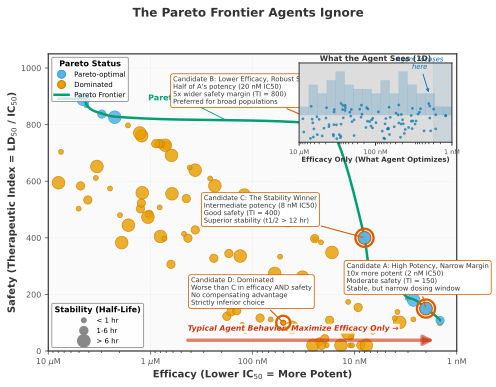
\includegraphics[width=\textwidth]{figures/fig6-pareto-frontier.jpeg}
\caption{The Pareto Frontier Agents Ignore. Two-dimensional scatter plot of candidate compounds across efficacy (IC50) and safety (LD50 ratio), with stability (half-life) encoded by point size. The Pareto frontier curve identifies candidates where improving one objective requires degrading another. Annotations show real decision trade-offs: lower efficacy but much safer, highly effective but stability concerns. Current single-objective optimization (red arrow pointing to maximum efficacy) misses this complexity.}
\label{fig:pareto}
\end{figure}

Pareto optimization is the appropriate framework. A candidate is Pareto-optimal if no other improves one objective without degrading another. The Pareto frontier is a curve (two objectives) or surface (three+). Practitioners navigate this frontier based on context.

Frontier visualization reveals trade-off structure. Steep regions require large sacrifices for modest gains; flat regions allow improvements with minimal cost. Clusters suggest distinct strategies (high-potency narrow-margin versus moderate-potency wide-margin). Gaps reveal unexplored regions.

Constructing the frontier requires multi-objective optimization. NSGA-II maintains candidate populations and selects non-dominated solutions. Multi-objective Bayesian optimization models objectives, selects candidates via acquisition functions balancing exploration and Pareto improvement, and updates with experimental results. These require tight integration between generative models, predictive models, and optimizers, which agents do not support.

Standalone multi-objective tools are advancing. PMMG \citep{pmmg2025} uses Pareto-guided Monte Carlo Tree Search to generate molecules satisfying seven simultaneous objectives with a 51.65\% success rate, outperforming baselines by 2.5 times. CheapVS \citep{cheapvs2025} enables human-guided preferential multi-objective Bayesian optimization, allowing chemists to express trade-off preferences via pairwise comparisons. These are effective optimization algorithms, but they are not integrated into agentic workflows providing uncertainty quantification, sensitivity analysis, stage-adaptive recommendations, and interactive decision support across iterative design cycles.

Constraints add complexity: synthesizability, solubility, permeability, absence of toxicophores. Constrained optimization identifies the Pareto frontier within feasible regions, which may be disjoint or conflicting. In peptide design, synthesis feasibility is often binding. Sequences with non-natural residues may be predicted optimal but are unavailable or prohibitively expensive. Regioselective cyclization can be unfeasible. Practitioners must balance optimization with synthetic pragmatism.

\subsubsection{Incorporating Uncertainty and Risk}

Predictions include uncertainty. IC50 equals 10 nM might have a 95% interval of 5-20 nM or 1-100 nM. Ignoring uncertainty leads to poor decisions: selecting high predicted activity with wide uncertainty and failing in validation. Incorporating uncertainty into multi-objective decisions is a standard requirement in Bayesian decision theory but is absent from current agents.

Bayesian optimization handles uncertainty via Gaussian processes providing means and variances. Acquisition functions (expected improvement, upper confidence bound) balance exploitation and exploration. Over rounds, uncertainty shrinks in explored regions and stays high elsewhere. Visualizing uncertainty to guide exploration versus exploitation is a key capability gap.

Risk profiles vary by stage. Early discovery tolerates high-risk, high-reward candidates. Late-stage demands well-characterized properties and high confidence. Effective frameworks would adapt recommendations accordingly.

In peptide pipelines, early rounds prioritized diversity, middle rounds balanced exploration and exploitation, final rounds focused on de-risking. This requires dynamic acquisition functions and explicit risk management absent from agents.

Sensitivity analysis is missing. How robust are rankings to model error? If bioactivity predictions have 20% error or toxicity is biased optimistic, which candidates remain Pareto-optimal? Sensitivity analysis quantifies robustness and guides resource allocation.

\subsubsection{Derived Requirements}

Closing this gap requires multi-objective Bayesian optimization with constraint handling, Pareto frontier visualization with interactive filtering, uncertainty quantification providing epistemic uncertainty in bioactivity prediction and dose-response confidence bands, and risk-aware candidate selection that adapts recommendations to development stage. The gap analysis identifies Pareto frontier representation, uncertainty quantification, risk-aware decision support, and structured decision spaces as design requirements, replacing the current pattern of outputting single optima.


\section{Design Requirements for Next-Generation Frameworks}
\label{sec:requirements}

The gaps identified in the preceding analysis reflect architectural assumptions that limit current frameworks. This section synthesizes five design requirements derived from the gap analysis and illustrates them with concrete use cases.

\subsection{Requirements Derived from Gap Analysis}

\subsubsection{Requirement 1: Multi-Paradigm Orchestration}

Closing Gap 3 requires support for ML training, RL, simulation, and optimization as first-class primitives. Effective frameworks would allow practitioners to specify workflows declaratively and receive an executable workflow graph supporting parallelization, checkpointing, and branching when validation fails. Human-in-the-loop decision points need to be explicit when models trade off accuracy, calibration, or interpretability. Workflow orchestration systems (Airflow, Kubeflow, Nextflow) already provide these abstractions; what is missing is tight integration with agent reasoning and iterative improvement.

\subsubsection{Requirement 2: Modality-Aware Representations}

Closing Gap 1 requires first-class support for peptides, proteins, and other modalities, not just small molecules. This entails PLM fine-tuning pipelines, structural biology integration (AlphaFold, flexible docking, molecular dynamics), and peptide-specific property prediction (aggregation, protease resistance, immunogenicity). Modality awareness would flow through data loaders, feature extractors, generative models, and evaluation metrics. Contextual tool selection would default peptides to ESM-2 embeddings and protein structures to structural alignment, rather than SMILES-based similarity.

\subsubsection{Requirement 3: In Vivo-In Silico Data Fusion}

Closing Gap 2 requires temporal modeling for longitudinal efficacy and safety data, multi-modal fusion (behavior, imaging, transcriptomics), and causal inference for mechanistic hypotheses. This entails bioinformatics pipelines (RNA-seq alignment, differential expression, pathway enrichment), computer vision, and statistical models for dose-response and mixed effects. Predictive efficacy modeling would align heterogeneous timepoints, handle missing data, and validate on temporally ordered splits. Mechanistic inference would integrate KEGG, GO, and Reactome to translate results into hypotheses and validation experiments.

\subsubsection{Requirement 4: Data-Efficient Learning}

Closing Gap 4 requires optimization for few-shot adaptation, active learning, and knowledge transfer across related tasks. This entails meta-learning, Bayesian uncertainty quantification, and transfer pipelines combining public pre-training (UniProt, PDB, ChEMBL) with private fine-tuning. Effective frameworks would recommend strategies based on dataset size: deep nets for 500 examples, simpler models for 50, few-shot for 10. Active learning loops would select candidates via acquisition functions, update models with experimental feedback, and signal when marginal information gain is low.

\subsubsection{Requirement 5: Multi-Objective, Risk-Aware Optimization}

Closing Gap 5 requires Pareto optimization with constraints, uncertainty quantification, sensitivity analysis, and interactive trade-off visualization. Results would take the form of Pareto frontiers with confidence intervals, constraint status, and robustness scores. Practitioners would filter by feasibility, adjust objective weights, and highlight low-uncertainty candidates. Risk-aware systems would adapt recommendations to stage: early exploration versus late-stage de-risking.

\subsection{Illustrative Use Cases}

These requirements imply a shift from chat-first tooling to workflow-first systems. Agents would maintain state across iterations, log decisions, and make assumptions explicit so practitioners can audit results and reproduce outcomes. This is a standard requirement in regulated environments and for teams that revisit decisions months later, often under new personnel or budget constraints.

To make these requirements concrete, we describe three representative use cases that current agents cannot handle but next-generation systems should support.

\subsubsection{Use Case 1: Peptide Lead Optimization}

\textbf{Input:} Fifty peptides with four assay endpoints, receptor structure, synthesis constraints.

\textbf{Workflow:} Fine-tune ESM-2, train multi-task regressor, use it as RL reward, filter by synthesis feasibility and stability, dock top candidates, cluster binding modes, present activity versus safety Pareto frontier with uncertainty.

\textbf{Output:} Ten synthesis candidates with rationales and confidence intervals.

\textbf{Human decisions:} Select among Pareto-optimal candidates based on strategic priorities and budget.

\subsubsection{Use Case 2: In Vivo Efficacy Prediction}

\textbf{Input:} In vitro assays and early in vivo markers for 20 peptides; predict day 28 outcomes.

\textbf{Workflow:} Normalize features, align temporal data with missing values, train regression models with stratified validation, identify early predictors and mechanistic drivers.

\textbf{Output:} Day 28 predictions with uncertainty and mechanistic hypotheses.

\textbf{Human decisions:} Choose peptides for full validation and whether to collect additional early markers.

\subsubsection{Use Case 3: Multi-Endpoint Assay Analysis}

\textbf{Input:} Four-endpoint data for 100 peptides.

\textbf{Workflow:} Normalize, cluster, validate stability, extract enriched sequence motifs, run pathway enrichment, visualize clusters.

\textbf{Output:} Distinct activity profile clusters with mechanistic hypotheses and selection recommendations.

\textbf{Human decisions:} Validate hypotheses and decide whether to focus on a single cluster or maintain diversity.

\subsection{Infrastructure Considerations}

\begin{table}[htbp]
\centering
\caption{Gap-to-Requirement Mapping: Priority Matrix for Next-Generation Agent Features}
\label{tab:requirement-priority}
\small
\begin{tabular}{lcccp{3cm}}
\hline
\textbf{Feature} & \textbf{Impact} & \textbf{Difficulty} & \textbf{Who Needs It} & \textbf{Priority} \\
\hline
Multi-paradigm orchestration & High & High & All & Critical \\
PLM fine-tuning pipelines & High & Medium & Biologics & Critical \\
Active learning loops & High & Medium & Small biotech & Critical \\
Pareto frontier visualization & High & Medium & All & High \\
Uncertainty quantification & High & Medium & All & High \\
In vivo data integration & High & High & All & High \\
Batch-mode workflows & Medium & Low & Small biotech & Medium \\
Transfer learning support & High & Medium & Small biotech & High \\
Constraint satisfaction & Medium & Medium & All & Medium \\
Workflow checkpointing & Low & Low & All & Medium \\
\hline
\end{tabular}
\end{table}

Realizing these capabilities requires infrastructure beyond current agents. API standards would need to cover PLMs (embedding extraction, fine-tuning, uncertainty), structural biology tools (AlphaFold, docking, molecular dynamics), and bioinformatics pipelines (alignment, differential expression, pathway enrichment). Version-controlled datasets, model registries, and provenance tracking are standard requirements for reproducibility and auditability.

Organizational alignment matters. Systems targeting small biotech contexts would need to fit modest compute budgets, minimal storage, and lightweight deployment. Documentation targeting non-ML-expert biologists would lower adoption barriers. Integration with existing tools (GraphPad, FlowJo, ImageJ, R/Bioconductor) avoids workflow disruption.


\section{Discussion}
\label{sec:discussion}

\subsection{Scope and Limitations}

The 15 task classes evaluated in this analysis are derived from peptide therapeutics development at a small biotech. While we expect many findings to generalize to other biologics (antibodies, nucleic acid therapeutics) and resource-constrained settings, applicability to these modalities requires further evaluation. The specific challenges of antibody CDR optimization, mRNA design, or gene therapy vector engineering may surface additional gaps not captured here.

Our three-level capability assessment (full support, partial support, not supported) captures more nuance than a binary scheme but may still oversimplify. The 0.5 weighting assigned to partial support is a modeling choice; alternative weightings could shift coverage scores. Some frameworks provide functionality that falls short of full workflow integration but represents meaningful progress. Where we identified partial support, we documented the specific capabilities and limitations in Appendix~\ref{sec:appendix-b}, but a more granular scoring framework could reveal additional nuance.

The field is rapidly evolving. Since beginning this analysis, systems like Agentomics \citep{agentomics2026} and ML-Agent \citep{mlagent2025} have demonstrated single-paradigm ML automation, and tools like PepTune \citep{peptune2024} and PepMLM \citep{pepmlm2025} have advanced peptide-specific generation. These developments address individual capabilities but do not yet close the integration gaps we identify.

\subsection{Relation to Existing Work}

This analysis complements two distinct contributions in the field. Seal et al. \citep{seal2025aiagents} provide a comprehensive architectural survey cataloging agent designs, tool integrations, and benchmarks. Their work maps what exists; ours evaluates what is missing when these systems confront diverse real-world requirements. The gaps we characterize are precisely the ones their survey catalogs but does not critique.

He et al. \citep{he2026chatinvent} demonstrate a deep single-organization deployment at AstraZeneca, establishing that agentic systems can deliver value in practice. However, their evaluation reflects one organizational context with extensive resources. Our analysis extends this by assessing generalizability across resource levels, data modalities, and therapeutic modalities.

Lakhan \citep{lakhan2025agentic} advocates for agentic AI adoption in biopharma. The adoption they advocate requires the design requirements identified in this analysis; without addressing the identified gaps, adoption will remain limited to settings that match current framework assumptions.

\subsection{Future Directions}

Three directions would advance the field. First, empirical benchmarks reflecting diverse drug discovery contexts beyond molecular generation. Current benchmarks (MoleculeNet, GuacaMol, Therapeutic Data Commons) focus on small-molecule property prediction and generation. Benchmarks incorporating peptide design, in vivo modeling, multi-modal integration, and resource-constrained settings would enable more representative framework evaluation.

Second, open-source multi-paradigm orchestration frameworks. Workflow orchestration systems (Airflow, Kubeflow, Nextflow) provide task graphs, dependency resolution, and resource allocation. Integrating agent reasoning with these systems, enabling inspection, diagnosis, and iterative improvement, would close the gap between workflow automation and intelligent orchestration.

Third, community-driven task class definitions spanning therapeutic modalities. Our 15 task classes reflect one practitioner's experience. Broader community input would extend coverage to antibodies, cell therapies, gene therapies, and other modalities, creating a shared evaluation framework for the field.

The appropriate design target is systems that augment practitioner judgment, not replace it. Drug discovery is too complex and context-dependent for full automation. Computational partners that handle preprocessing, training, tuning, and visualization while practitioners focus on hypotheses, mechanistic interpretation, and strategic trade-offs represent the appropriate design target. Partnership requires bidirectional communication: agents explain reasoning, expose assumptions, and quantify uncertainty; practitioners provide feedback and correct errors.


\section{Conclusion}
\label{sec:conclusion}

We evaluated six agentic frameworks against 15 drug discovery task classes and identified five critical capability gaps: small-molecule representation bias, absence of in vivo-in silico integration, limited computational paradigm support, misalignment with small-biotech constraints, and single-objective optimization assumptions. These gaps reflect architectural constraints that individual feature additions do not address: closing them requires changes to core framework design.
Our knowledge probing experiment reinforces this conclusion: four frontier LLMs
demonstrate competent peptide reasoning across all categories tested, yet this expertise
remains stranded behind agent architectures that provide no peptide-aware tools or
sequence-native workflows.

From the identified gaps, we derived five design requirements for next-generation frameworks: multi-paradigm orchestration supporting ML training, RL, and simulation as first-class primitives; modality-aware representations for peptides, proteins, and biologics; in vivo data integration with temporal modeling and multi-modal fusion; data-efficient learning through few-shot adaptation, active learning, and transfer learning; and multi-objective, risk-aware optimization with Pareto frontiers and uncertainty quantification.

The capability matrix and derived requirements provide a roadmap for framework developers and a benchmarking tool for practitioners evaluating agentic systems against their specific discovery contexts. Progress since 2023 has established what agentic systems can achieve. The next phase will determine whether these systems generalize beyond small-molecule workflows at well-resourced organizations to become core infrastructure for drug discovery broadly.


\appendix
\section{Task Class Descriptions}
\label{appendix:task-classes}

This appendix provides full descriptions of the 15 task classes used in our evaluation, including representative inputs, outputs, computational requirements, and evaluation criteria. Task classes are derived from real-world drug discovery workflows spanning peptide therapeutics, in vivo pharmacology, and computational biology.

\begin{enumerate}[leftmargin=*, label=\textbf{T\arabic*.}]

\item \textbf{ML bioactivity prediction (multi-endpoint regression).}
Train supervised models predicting multiple biological endpoints (e.g., proliferation, migration, secretion, toxicity) from peptide features. \\
\textit{Inputs:} Peptide sequences or descriptors (50--500 compounds), multi-endpoint assay measurements. \\
\textit{Outputs:} Predictive models with per-endpoint performance metrics and uncertainty estimates. \\
\textit{Requirements:} Feature extraction (sequence-based or PLM embeddings), stratified cross-validation, hyperparameter tuning, multi-task or multi-output regression, calibration. \\
\textit{Evaluation:} Per-endpoint $R^2$, RMSE, calibration error, cross-validated confidence intervals.

\item \textbf{Generative peptide design (PLM fine-tuning).}
Fine-tune protein language models on therapeutic sequences for conditional de novo peptide generation. \\
\textit{Inputs:} Training set of therapeutic peptide sequences (50--500), target property constraints. \\
\textit{Outputs:} Novel peptide sequences satisfying property constraints with diversity metrics. \\
\textit{Requirements:} PLM fine-tuning (ProtGPT2, ProtBERT), transfer learning, sampling with temperature control, property filtering, novelty and diversity assessment. \\
\textit{Evaluation:} Validity, novelty, diversity, predicted property distributions, KL divergence from training set.

\item \textbf{Peptide-receptor binding site analysis and clustering.}
Analyze peptide-receptor interactions through flexible docking, cluster by binding region, and correlate with bioactivity. \\
\textit{Inputs:} Peptide sequences, receptor structure (experimental or AlphaFold-predicted), bioactivity data. \\
\textit{Outputs:} Binding mode clusters, per-cluster activity profiles, key interacting residues. \\
\textit{Requirements:} Conformational sampling, flexible docking, interaction fingerprinting, clustering, statistical correlation with bioactivity. \\
\textit{Evaluation:} Cluster separation (silhouette score), activity-cluster correlation (ANOVA), docking score convergence.

\item \textbf{In vivo recovery modeling (longitudinal clinical scores).}
Model longitudinal clinical outcomes from animal studies to identify temporal efficacy signatures and classify treatment responses. \\
\textit{Inputs:} Time-series clinical scores (e.g., motor coordination assessments at days 1, 3, 7, 14, 28), treatment groups, covariates. \\
\textit{Outputs:} Temporal efficacy profiles, responder/non-responder classification, predictive early markers. \\
\textit{Requirements:} Mixed-effects models, time-series classification, missing data imputation, temporal feature engineering, bootstrap confidence intervals. \\
\textit{Evaluation:} Classification accuracy (responder vs non-responder), prediction of late outcomes from early markers ($R^2$, AUC).

\item \textbf{Peptide-enzyme interaction modeling for stability optimization.}
Predict protease cleavage sites and design modifications that improve serum stability while preserving bioactivity. \\
\textit{Inputs:} Peptide sequences, known half-life measurements, protease specificity data. \\
\textit{Outputs:} Predicted cleavage sites, suggested stabilizing modifications, stability-activity trade-off analysis. \\
\textit{Requirements:} Sequence-based cleavage prediction across protease families, molecular modeling of modifications (D-amino acids, cyclization, PEGylation), multi-objective balancing of stability and affinity. \\
\textit{Evaluation:} Cleavage site prediction accuracy, correlation of predicted vs measured half-life, activity retention after modification.

\item \textbf{Protein language model-based receptor type prediction.}
Classify peptide sequences by receptor type using PLM embeddings and supervised learning. \\
\textit{Inputs:} Peptide sequences with receptor type labels (50--200 labeled examples), pre-trained PLM (ESM-2). \\
\textit{Outputs:} Multi-class classifier with per-class probabilities and uncertainty estimates. \\
\textit{Requirements:} PLM embedding extraction, layer selection, classifier training (logistic regression, gradient-boosted trees), cross-validation, calibration. \\
\textit{Evaluation:} Multi-class AUC-ROC, precision-recall per class, calibration curves, confusion matrix.

\item \textbf{Monte Carlo optimization for peptide landscape exploration.}
Explore peptide sequence space using stochastic optimization to balance exploitation of known active regions with exploration of novel regions. \\
\textit{Inputs:} Initial peptide set, fitness function (bioactivity predictor), sequence constraints. \\
\textit{Outputs:} Optimized peptide set with diversity metrics, landscape topology characterization. \\
\textit{Requirements:} Metropolis-Hastings sampling, acceptance criteria tuning, fitness landscape estimation, convergence diagnostics, diversity maintenance. \\
\textit{Evaluation:} Best fitness achieved, sequence diversity (edit distance distribution), convergence rate, landscape coverage.

\item \textbf{RNA sequencing and single-cell transcriptomics analysis.}
Process bulk or single-cell RNA-seq data to identify differentially expressed genes, cell-type compositions, and treatment-responsive pathways. \\
\textit{Inputs:} FASTQ files or count matrices, experimental design (treatment vs control, time points). \\
\textit{Outputs:} Differentially expressed gene lists, pathway enrichment results, cell-type annotations (scRNA-seq), pseudotime trajectories. \\
\textit{Requirements:} Read alignment (STAR, HISAT2), quantification, normalization (DESeq2, edgeR), dimensionality reduction (UMAP, t-SNE), clustering, trajectory inference, pathway enrichment (GSEA, KEGG, GO). \\
\textit{Evaluation:} Alignment rates, library complexity, differential expression FDR control, biological coherence of enriched pathways.

\item \textbf{Digital image processing for tissue quantification.}
Extract quantitative morphometric features from tissue imaging (histology, radiographic imaging) for treatment efficacy assessment. \\
\textit{Inputs:} Tissue images, region-of-interest annotations, treatment group labels. \\
\textit{Outputs:} Quantified tissue features (area, density, gap measurements), statistical comparisons across treatment groups. \\
\textit{Requirements:} Image preprocessing (contrast normalization, artifact removal), segmentation (thresholding or learned), feature extraction, automated ROI detection, statistical testing. \\
\textit{Evaluation:} Segmentation accuracy (Dice coefficient), inter-rater agreement, effect size and statistical significance of treatment differences.

\item \textbf{Immune response profiling (pathway analysis).}
Characterize immune modulation by analyzing pathway activation, upstream regulators, and inflammatory scoring from transcriptomic or proteomic data. \\
\textit{Inputs:} Expression data (genes or proteins), treatment conditions, reference pathway databases. \\
\textit{Outputs:} Activated/suppressed pathways, upstream regulator predictions, inflammatory response scores. \\
\textit{Requirements:} Pathway enrichment (GSEA, IPA-style analysis), upstream regulator inference, network construction, scoring metrics for inflammatory vs anti-inflammatory balance. \\
\textit{Evaluation:} Pathway enrichment FDR, consistency across methods, biological plausibility of upstream regulators.

\item \textbf{Functional annotation and pathway enrichment.}
Annotate gene or protein lists with functional categories (GO terms, KEGG pathways) and identify statistically enriched biological processes. \\
\textit{Inputs:} Gene/protein lists from differential expression or clustering, background gene set, annotation databases. \\
\textit{Outputs:} Enriched GO terms and KEGG pathways with p-values, gene network visualizations. \\
\textit{Requirements:} GO/KEGG annotation retrieval, hypergeometric or Fisher enrichment testing, multiple testing correction, network construction (STRING, Cytoscape). \\
\textit{Evaluation:} Enrichment significance after correction, semantic coherence of enriched terms, overlap with known biology.

\item \textbf{Computer vision for behavioral phenotyping.}
Apply pose estimation and tracking to animal behavioral videos to quantify treatment effects on social behavior, motor function, or anxiety-like phenotypes. \\
\textit{Inputs:} Behavioral videos (multiple animals per session), body part definitions, treatment group assignments. \\
\textit{Outputs:} Tracked keypoint trajectories, derived behavioral metrics, statistical comparisons. \\
\textit{Requirements:} Pose estimation model training (DeepLabCut), tracking validation, time-series feature engineering, behavioral metric computation, statistical testing with repeated measures. \\
\textit{Evaluation:} Tracking accuracy (pixel error), behavioral metric reliability (test-retest), effect size and significance of treatment differences.

\item \textbf{Predictive modeling bridging in vivo and in vitro endpoints.}
Develop composite efficacy metrics that correlate in vitro bioactivity with long-term in vivo outcomes to enable early candidate prioritization. \\
\textit{Inputs:} In vitro assay data (multiple endpoints), early and late in vivo measurements, compound identifiers. \\
\textit{Outputs:} Predictive efficacy model, feature importance rankings, predicted long-term outcomes with confidence intervals. \\
\textit{Requirements:} Multi-source feature extraction, temporal alignment, imputation, regression or classification modeling, stratified cross-validation on temporally ordered splits. \\
\textit{Evaluation:} Prediction accuracy ($R^2$, AUC for classification), early marker predictive power, model stability across cross-validation folds.

\item \textbf{Reinforcement learning for de novo peptide generation.}
Optimize peptide sequences using RL with multi-objective reward functions combining bioactivity, stability, and diversity. \\
\textit{Inputs:} Pre-trained generative model (ProtGPT2), reward model(s) for bioactivity and stability, diversity constraints. \\
\textit{Outputs:} Optimized peptide sequences with reward decomposition, diversity statistics, training curves. \\
\textit{Requirements:} Policy optimization (PPO, GRPO variants), reward model training, KL regularization against reference policy, curriculum learning (staged reward introduction), diversity penalties. \\
\textit{Evaluation:} Mean reward, reward component distributions, sequence diversity, KL divergence from reference, mode collapse indicators.

\item \textbf{Safety and toxicology modeling (dose-response, multi-objective trade-offs).}
Model dose-response relationships accounting for repeated measures and time-dependent effects, and navigate safety-efficacy trade-offs for candidate selection. \\
\textit{Inputs:} Dose-response data (multiple doses, time points, endpoints), efficacy measurements, compound properties. \\
\textit{Outputs:} Dose-response curves with confidence bands, therapeutic window estimates, Pareto frontier of safety vs efficacy. \\
\textit{Requirements:} Generalized linear mixed models, repeated measures analysis, LD50/ED50 estimation with confidence intervals, multi-objective optimization, Pareto frontier construction, species translation modeling. \\
\textit{Evaluation:} Model fit (AIC/BIC), confidence interval coverage, Pareto frontier hypervolume, robustness of therapeutic window estimates.

\end{enumerate}

\section{Detailed Capability Matrix}
\label{sec:appendix-b}

This appendix extends the capability matrix (Table~\ref{tab:capability-matrix}) with per-dimension assessments for each framework. Each framework is evaluated across the five dimensions defined in \S\ref{sec:methods}: molecular representation (D1), computational paradigm support (D2), data modality integration (D3), resource assumptions (D4), and optimization framework (D5). Assessments are based on published documentation, available source code, and demonstrated use cases as of early 2026.

\subsection{ChemCrow}

ChemCrow \citep{bran2024chemcrow} orchestrates 18 chemistry tools via GPT-4, including RDKit for molecular property calculation, PubChem for compound lookup, and reaction prediction APIs for retrosynthesis.

\begin{table}[htbp]
\centering
\caption{ChemCrow: Per-Dimension Assessment}
\label{tab:chemcrow-detail}
\small
\begin{tabular}{lcp{8cm}}
\toprule
\textbf{Dimension} & \textbf{Rating} & \textbf{Evidence and Notes} \\
\midrule
D1: Molecular repr. & \psup & Supports SMILES and molecular fingerprints via RDKit. No peptide sequence representations, PLM embeddings, or conformational sampling. \\
D2: Comp. paradigm & \nsup & Tool invocation only (stateless API calls). No ML training, RL, or simulation orchestration. \\
D3: Data modality & \nsup & Text and SMILES inputs only. No imaging, time-series, transcriptomics, or behavioral data support. \\
D4: Resource assumptions & \psup & Lightweight tool calls; does not require HPC. However, no few-shot, active learning, or transfer learning support. \\
D5: Optimization & \nsup & Single-objective property optimization. No Pareto frontiers, constraint satisfaction, or uncertainty quantification. \\
\bottomrule
\end{tabular}
\end{table}

\noindent\textbf{Partial support details.} Task 3 (peptide-receptor binding): ChemCrow includes docking tools designed for small-molecule rigid-body screening; these do not handle peptide conformational flexibility or induced-fit binding. Task 15 (safety/toxicology): includes toxicophore detection and basic ADMET prediction for small molecules but lacks dose-response modeling, mixed-effects analysis, or multi-objective trade-off reasoning.

\subsection{Coscientist}

Coscientist \citep{boiko2023coscientist} autonomously plans and executes chemical syntheses by interfacing with laboratory automation, web search, and code execution.

\begin{table}[htbp]
\centering
\caption{Coscientist: Per-Dimension Assessment}
\label{tab:coscientist-detail}
\small
\begin{tabular}{lcp{8cm}}
\toprule
\textbf{Dimension} & \textbf{Rating} & \textbf{Evidence and Notes} \\
\midrule
D1: Molecular repr. & \nsup & Designed for small-molecule organic synthesis. No peptide or protein representations. \\
D2: Comp. paradigm & \nsup & Code execution capability exists but is used for synthesis protocol generation, not ML training or RL. \\
D3: Data modality & \nsup & Text and structured chemical data only. No in vivo, imaging, or transcriptomic data handling. \\
D4: Resource assumptions & \psup & Operates with standard compute but assumes access to automated laboratory equipment (Emerald Cloud Lab). \\
D5: Optimization & \nsup & Optimizes synthesis yield as a single objective. No multi-objective framework. \\
\bottomrule
\end{tabular}
\end{table}

\noindent\textbf{Coverage: 0/15 task classes.} Coscientist's strength lies in closed-loop synthesis execution, a capability orthogonal to the 15 task classes evaluated here, which focus on computational modeling rather than laboratory automation.

\subsection{PharmAgents}

PharmAgents \citep{gao2025pharmagents} deploys specialized LLM agents for target identification, compound screening, and interaction prediction, coordinated through a multi-agent architecture with knowledge graph integration.

\begin{table}[htbp]
\centering
\caption{PharmAgents: Per-Dimension Assessment}
\label{tab:pharmagents-detail}
\small
\begin{tabular}{lcp{8cm}}
\toprule
\textbf{Dimension} & \textbf{Rating} & \textbf{Evidence and Notes} \\
\midrule
D1: Molecular repr. & \psup & Supports SMILES and molecular graphs. Knowledge graph includes protein targets but no PLM-based peptide representations. \\
D2: Comp. paradigm & \psup & Invokes pre-trained predictors for property estimation. No model training, fine-tuning, or RL support. \\
D3: Data modality & \psup & Structured databases and knowledge graphs. Pathway-level information available but not computational enrichment pipelines. \\
D4: Resource assumptions & \nsup & Assumes large compound libraries and knowledge graph infrastructure typical of large pharma. \\
D5: Optimization & \nsup & Rank-based compound selection. No Pareto optimization or uncertainty quantification. \\
\bottomrule
\end{tabular}
\end{table}

\noindent\textbf{Partial support details.} Task 1 (ML bioactivity): can invoke pre-trained models for single-endpoint prediction but cannot train multi-endpoint regressors on proprietary data. Tasks 10--11 (immune profiling, functional annotation): knowledge graph queries return pathway-level information but do not perform computational enrichment analysis (GSEA, hypergeometric testing). Task 15 (safety): includes ADMET prediction modules for small molecules.

\subsection{ChatInvent}

ChatInvent \citep{he2026chatinvent} was deployed at AstraZeneca over 13 months for literature-driven molecular design and synthesis planning, with access to institutional databases and computational infrastructure.

\begin{table}[htbp]
\centering
\caption{ChatInvent: Per-Dimension Assessment}
\label{tab:chatinvent-detail}
\small
\begin{tabular}{lcp{8cm}}
\toprule
\textbf{Dimension} & \textbf{Rating} & \textbf{Evidence and Notes} \\
\midrule
D1: Molecular repr. & \psup & Supports SMILES-based molecular design and literature-based structure analysis. No peptide-specific representations or PLMs. \\
D2: Comp. paradigm & \nsup & LLM reasoning over literature and molecular design tools. No ML training, RL, or simulation. \\
D3: Data modality & \psup & Literature text, molecular structures, and internal databases. No in vivo data, imaging, or transcriptomics. \\
D4: Resource assumptions & \nsup & Designed for AstraZeneca-scale resources: institutional literature access, HPC, large proprietary databases, specialized teams. \\
D5: Optimization & \nsup & Literature-guided hypothesis generation. No formal multi-objective optimization or uncertainty quantification. \\
\bottomrule
\end{tabular}
\end{table}

\noindent\textbf{Partial support details.} Tasks 10--11 (immune profiling, functional annotation): literature synthesis can surface pathway-level knowledge but does not perform computational analysis. Task 15 (safety): can retrieve safety-related literature and flag known liabilities from text; no quantitative dose-response modeling.

\subsection{MADD}

MADD \citep{madd2025} coordinates multiple LLM agents for molecular design, property prediction, and docking in a multi-agent collaboration framework.

\begin{table}[htbp]
\centering
\caption{MADD: Per-Dimension Assessment}
\label{tab:madd-detail}
\small
\begin{tabular}{lcp{8cm}}
\toprule
\textbf{Dimension} & \textbf{Rating} & \textbf{Evidence and Notes} \\
\midrule
D1: Molecular repr. & \psup & Supports SMILES-based molecular generation and property prediction. No peptide or protein representations. \\
D2: Comp. paradigm & \psup & Multi-agent coordination for design-predict-dock cycles. Agents invoke tools but do not train models or run RL. \\
D3: Data modality & \nsup & Molecular structures and predicted properties only. No in vivo, imaging, or transcriptomic data. \\
D4: Resource assumptions & \psup & Moderate compute requirements for docking. Does not assume pharma-scale databases but lacks few-shot or active learning. \\
D5: Optimization & \nsup & Iterative design refinement toward single objectives. No Pareto optimization or constraint satisfaction. \\
\bottomrule
\end{tabular}
\end{table}

\noindent\textbf{Partial support details.} Task 1 (ML bioactivity): prediction agents can estimate properties but from pre-trained models, not trained on proprietary data. Task 3 (peptide-receptor binding): includes docking workflows designed for small molecules. Task 15 (safety): property prediction agents can flag liabilities but without multi-objective reasoning.

\subsection{DiscoVerse}

DiscoVerse \citep{discoverse2025} provides multi-agent pharmaceutical workflow automation with traceable reasoning, developed by Roche-affiliated researchers.

\begin{table}[htbp]
\centering
\caption{DiscoVerse: Per-Dimension Assessment}
\label{tab:discoverse-detail}
\small
\begin{tabular}{lcp{8cm}}
\toprule
\textbf{Dimension} & \textbf{Rating} & \textbf{Evidence and Notes} \\
\midrule
D1: Molecular repr. & \psup & Supports small-molecule representations and reverse translation workflows. Limited protein or peptide support. \\
D2: Comp. paradigm & \psup & Workflow automation with traceability. Orchestrates existing tools but does not support model training or RL. \\
D3: Data modality & \psup & Integrates multiple data sources including clinical and preclinical information. Limited in vivo temporal modeling or imaging. \\
D4: Resource assumptions & \nsup & Designed for large pharma infrastructure and data availability. \\
D5: Optimization & \nsup & Workflow-driven decision support. No formal multi-objective optimization framework. \\
\bottomrule
\end{tabular}
\end{table}

\noindent\textbf{Partial support details.} Task 1 (ML bioactivity): workflow automation may include prediction steps using pre-trained models. Tasks 10--11 (immune profiling, functional annotation): reverse translation capability includes pathway-level reasoning from clinical observations. Task 15 (safety): clinical-preclinical integration provides safety context but lacks quantitative multi-objective optimization.

\subsection{Cross-Framework Summary}

Table~\ref{tab:dimension-summary} summarizes per-dimension coverage across all six frameworks. The sparsest dimensions, computational paradigm support (D2) and optimization framework (D5), reflect the deepest architectural limitations: LLM-as-orchestrator designs cannot support gradient-based training or multi-objective reasoning without fundamental changes.

\begin{table}[htbp]
\centering
\caption{Cross-Framework Dimension Coverage Summary. Fraction of frameworks providing full (\fsup) or partial (\psup) support per evaluation dimension.}
\label{tab:dimension-summary}
\small
\begin{tabular}{lccl}
\toprule
\textbf{Dimension} & \textbf{Full} & \textbf{Partial} & \textbf{Primary Limitation} \\
\midrule
D1: Molecular representation & 0/6 & 5/6 & No PLM or peptide-native support \\
D2: Computational paradigm & 0/6 & 3/6 & No ML training, RL, or simulation \\
D3: Data modality & 0/6 & 3/6 & No in vivo, imaging, or omics pipelines \\
D4: Resource assumptions & 0/6 & 3/6 & No few-shot, active learning, or transfer \\
D5: Optimization framework & 0/6 & 0/6 & No multi-objective or uncertainty support \\
\bottomrule
\end{tabular}
\end{table}


% Bibliography
\bibliography{references}

\end{document}
